% This file was created with matplot2tikz v0.4.2.
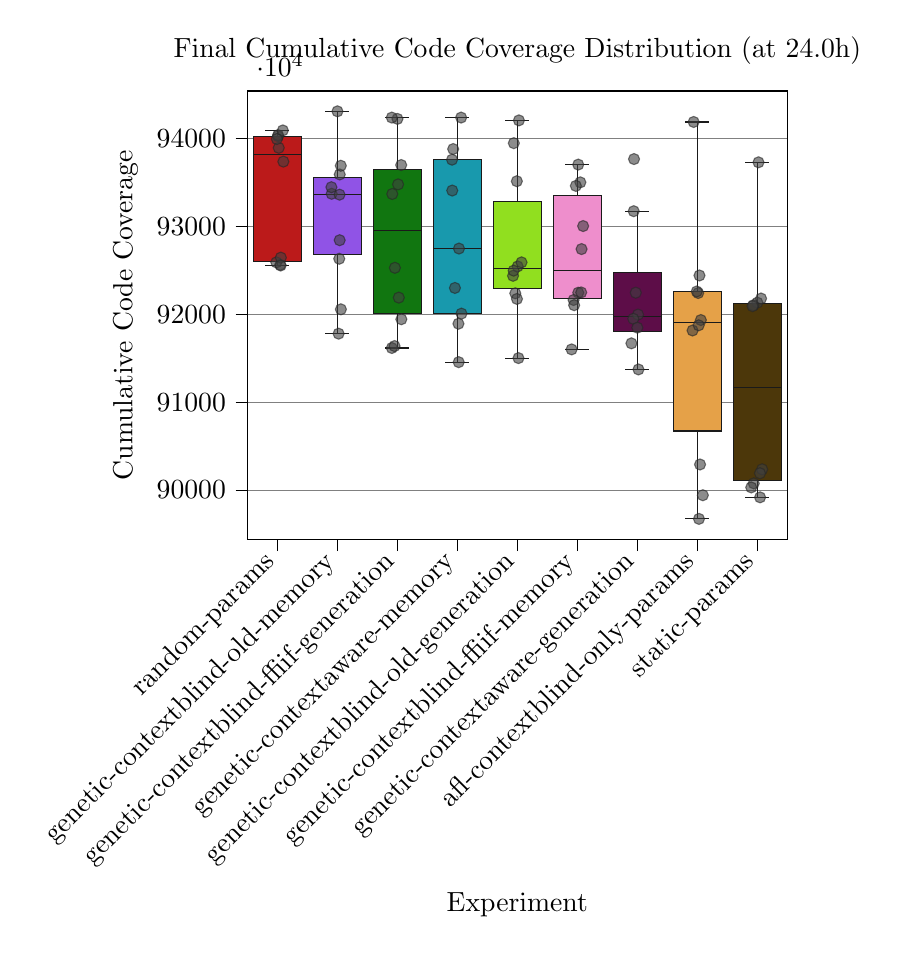
\begin{tikzpicture}

\definecolor{black26}{RGB}{26,26,26}
\definecolor{darkgray176}{RGB}{176,176,176}
\definecolor{darkolivegreen765510}{RGB}{76,55,10}
\definecolor{darkslategray38}{RGB}{38,38,38}
\definecolor{firebrick1872626}{RGB}{187,26,26}
\definecolor{gray}{RGB}{128,128,128}
\definecolor{green1711816}{RGB}{17,118,16}
\definecolor{indigo931372}{RGB}{93,13,72}
\definecolor{lightseagreen24153173}{RGB}{24,153,173}
\definecolor{mediumslateblue14483230}{RGB}{144,83,230}
\definecolor{plum238142204}{RGB}{238,142,204}
\definecolor{sandybrown22916172}{RGB}{229,161,72}
\definecolor{yellowgreen14522331}{RGB}{145,223,31}

\begin{axis}[
tick align=outside,
tick pos=left,
title={Final Cumulative Code Coverage Distribution (at 24.0h)},
x grid style={darkgray176},
xlabel={Experiment},
xmin=-0.5, xmax=8.5,
xtick style={color=black},
xtick={0,1,2,3,4,5,6,7,8},
xticklabel style={rotate=45.0,anchor=east},
xticklabels={
  random-params,
  genetic-contextblind-old-memory,
  genetic-contextblind-ffiif-generation,
  genetic-contextaware-memory,
  genetic-contextblind-old-generation,
  genetic-contextblind-ffiif-memory,
  genetic-contextaware-generation,
  afl-contextblind-only-params,
  static-params
},
y grid style={gray},
ylabel={Cumulative Code Coverage},
ymajorgrids,
ymin=89440.2, ymax=94539.8,
ytick style={color=black},
ytick={89000,90000,91000,92000,93000,94000,95000},
yticklabels={
  \num{89000},
  \num{90000},
  \num{91000},
  \num{92000},
  \num{93000},
  \num{94000},
  \num{95000}
}
]
\path [draw=black26, fill=firebrick1872626]
(axis cs:-0.4,92603.5)
--(axis cs:0.4,92603.5)
--(axis cs:0.4,94017)
--(axis cs:-0.4,94017)
--(axis cs:-0.4,92603.5)
--cycle;
\addplot [black26]
table {%
0 92603.5
0 92554
};
\addplot [black26]
table {%
0 94017
0 94091
};
\addplot [black26]
table {%
-0.2 92554
0.2 92554
};
\addplot [black26]
table {%
-0.2 94091
0.2 94091
};
\path [draw=black26, fill=mediumslateblue14483230]
(axis cs:0.6,92683.75)
--(axis cs:1.4,92683.75)
--(axis cs:1.4,93553.75)
--(axis cs:0.6,93553.75)
--(axis cs:0.6,92683.75)
--cycle;
\addplot [black26]
table {%
1 92683.75
1 91779
};
\addplot [black26]
table {%
1 93553.75
1 94308
};
\addplot [black26]
table {%
0.8 91779
1.2 91779
};
\addplot [black26]
table {%
0.8 94308
1.2 94308
};
\path [draw=black26, fill=green1711816]
(axis cs:1.6,92004.5)
--(axis cs:2.4,92004.5)
--(axis cs:2.4,93642)
--(axis cs:1.6,93642)
--(axis cs:1.6,92004.5)
--cycle;
\addplot [black26]
table {%
2 92004.5
2 91616
};
\addplot [black26]
table {%
2 93642
2 94237
};
\addplot [black26]
table {%
1.8 91616
2.2 91616
};
\addplot [black26]
table {%
1.8 94237
2.2 94237
};
\path [draw=black26, fill=lightseagreen24153173]
(axis cs:2.6,92007)
--(axis cs:3.4,92007)
--(axis cs:3.4,93758)
--(axis cs:2.6,93758)
--(axis cs:2.6,92007)
--cycle;
\addplot [black26]
table {%
3 92007
3 91455
};
\addplot [black26]
table {%
3 93758
3 94237
};
\addplot [black26]
table {%
2.8 91455
3.2 91455
};
\addplot [black26]
table {%
2.8 94237
3.2 94237
};
\path [draw=black26, fill=yellowgreen14522331]
(axis cs:3.6,92287.75)
--(axis cs:4.4,92287.75)
--(axis cs:4.4,93282.25)
--(axis cs:3.6,93282.25)
--(axis cs:3.6,92287.75)
--cycle;
\addplot [black26]
table {%
4 92287.75
4 91501
};
\addplot [black26]
table {%
4 93282.25
4 94205
};
\addplot [black26]
table {%
3.8 91501
4.2 91501
};
\addplot [black26]
table {%
3.8 94205
4.2 94205
};
\path [draw=black26, fill=plum238142204]
(axis cs:4.6,92182.75)
--(axis cs:5.4,92182.75)
--(axis cs:5.4,93345.75)
--(axis cs:4.6,93345.75)
--(axis cs:4.6,92182.75)
--cycle;
\addplot [black26]
table {%
5 92182.75
5 91600
};
\addplot [black26]
table {%
5 93345.75
5 93702
};
\addplot [black26]
table {%
4.8 91600
5.2 91600
};
\addplot [black26]
table {%
4.8 93702
5.2 93702
};
\path [draw=black26, fill=indigo931372]
(axis cs:5.6,91802.5)
--(axis cs:6.4,91802.5)
--(axis cs:6.4,92476.75)
--(axis cs:5.6,92476.75)
--(axis cs:5.6,91802.5)
--cycle;
\addplot [black26]
table {%
6 91802.5
6 91372
};
\addplot [black26]
table {%
6 92476.75
6 93172
};
\addplot [black26]
table {%
5.8 91372
6.2 91372
};
\addplot [black26]
table {%
5.8 93172
6.2 93172
};
\path [draw=black26, fill=sandybrown22916172]
(axis cs:6.6,90672)
--(axis cs:7.4,90672)
--(axis cs:7.4,92254.5)
--(axis cs:6.6,92254.5)
--(axis cs:6.6,90672)
--cycle;
\addplot [black26]
table {%
7 90672
7 89672
};
\addplot [black26]
table {%
7 92254.5
7 94187
};
\addplot [black26]
table {%
6.8 89672
7.2 89672
};
\addplot [black26]
table {%
6.8 94187
7.2 94187
};
\path [draw=black26, fill=darkolivegreen765510]
(axis cs:7.6,90104.75)
--(axis cs:8.4,90104.75)
--(axis cs:8.4,92124.75)
--(axis cs:7.6,92124.75)
--(axis cs:7.6,90104.75)
--cycle;
\addplot [black26]
table {%
8 90104.75
8 89917
};
\addplot [black26]
table {%
8 92124.75
8 93728
};
\addplot [black26]
table {%
7.8 89917
8.2 89917
};
\addplot [black26]
table {%
7.8 93728
8.2 93728
};
\addplot [black26]
table {%
-0.4 93814.5
0.4 93814.5
};
\addplot [black26]
table {%
0.6 93365
1.4 93365
};
\addplot [black26]
table {%
1.6 92948
2.4 92948
};
\addplot [black26]
table {%
2.6 92747
3.4 92747
};
\addplot [black26]
table {%
3.6 92520
4.4 92520
};
\addplot [black26]
table {%
4.6 92494.5
5.4 92494.5
};
\addplot [black26]
table {%
5.6 91972
6.4 91972
};
\addplot [black26]
table {%
6.6 91904
7.4 91904
};
\addplot [black26]
table {%
7.6 91164
8.4 91164
};
\addplot [draw=darkslategray38, fill=darkgray, mark=*, only marks, opacity=0.6]
table{%
x  y
0.0213510261722784 93893
0.0109844243782891 94025
0.0461057949611222 92563
0.0108822257353461 94038
-0.0186795915474005 92590
-0.00957042832141333 93993
0.0899097188663371 94091
0.0986395699802112 93736
0.0567624293480395 92644
0.0534494957346457 92554
};
\addplot [draw=darkslategray38, fill=darkgray, mark=*, only marks, opacity=0.6]
table{%
x  y
1.03777586637053 92842
1.0579926742743 92056
0.904357229276866 93370
1.03042378074396 92631
1.03566742768703 93360
1.03858325892715 93590
1.0566046191865 93689
1.00062120578307 94308
0.900076658879988 93445
1.02007914211426 91779
};
\addplot [draw=darkslategray38, fill=darkgray, mark=*, only marks, opacity=0.6]
table{%
x  y
2.00108973653332 94222
1.9079943858505 91616
2.06655363958428 91943
2.01168328107768 93477
1.90757567822081 94237
1.95874983821183 92528
2.02353320226319 92189
1.91536877408463 93368
1.95291185969491 91638
2.06382540774726 93697
};
\addplot [draw=darkslategray38, fill=darkgray, mark=*, only marks, opacity=0.6]
table{%
x  y
3.01865358467008 91892
3.06920864151084 92007
2.96010112738674 92299
2.91517569891575 93407
3.06337903215085 94237
3.02739290084635 92747
2.91189606346091 93758
2.93099066851356 93879
3.02299593072405 91455
};
\addplot [draw=darkslategray38, fill=darkgray, mark=*, only marks, opacity=0.6]
table{%
x  y
3.96662171611469 92238
4.02733006776964 94205
3.99438949561292 92174
3.9292745650469 92437
4.00666685523782 92544
3.9391617886485 92496
3.9927068091612 93513
4.07104497504235 92590
3.94232875496187 93946
4.01967075652024 91501
};
\addplot [draw=darkslategray38, fill=darkgray, mark=*, only marks, opacity=0.6]
table{%
x  y
5.0983046491584 93003
5.05213561805434 93500
5.01691948731763 92245
5.07205766864069 92741
4.90599808897949 91600
5.01642157097975 93702
5.06612371588447 92248
4.9770859858057 93460
4.9390221678345 92162
4.94823583478178 92103
};
\addplot [draw=darkslategray38, fill=darkgray, mark=*, only marks, opacity=0.6]
table{%
x  y
5.94674233357569 93765
6.02095223777989 91372
5.94192152597086 93172
6.01350385388443 91996
5.93509455316271 91948
6.0024792879528 91847
5.90359469325546 91669
5.97613326726118 92245
};
\addplot [draw=darkslategray38, fill=darkgray, mark=*, only marks, opacity=0.6]
table{%
x  y
7.03845109391167 92441
7.03009261813863 89672
6.9416213072983 94187
6.92319334284337 91815
7.06150037021612 91934
7.01709781483064 92241
7.0256355476461 91874
6.99317541615201 92259
7.09480815576882 89941
7.04823647420984 90291
};
\addplot [draw=darkslategray38, fill=darkgray, mark=*, only marks, opacity=0.6]
table{%
x  y
8.00470941566166 92132
8.02303102603304 93728
7.94375104076038 90076
8.08391406543061 90236
7.93937447575702 92103
8.04765616518359 90191
8.06573112592527 92179
7.90203628755679 90030
8.04949726519665 89917
7.92367126555698 92092
};
\end{axis}

\end{tikzpicture}
